Der findes flere forskellige former for programmer, der allerede helt eller delvist løser SMS-begrænsnings problemet. Vi vil i det følgende afsnit tage udgangspunkt i to eksisterende programmer.

Det første program hedder SMS ZIP, og det virker kun til smartphones med Windows phone 5 og 6 som operativsystem. Det er et forældet program, eftersom det kun virker på forældede platforme. Programmet har dog stadig relevans,  eftersom det er tanken bag programmet, der er interessant. Dette program er af typen ikke tabsfri, da det går ind og fjerner alle mellemrum i teksten, og erstatter første bogstav i følgende ord med et stort bogstav, således at teksten stadig kan læses. Ydermere er det programmeret til at kunne identificere bestemte ord, og så erstatte disse med forkortelser. Programmet er indrettet således, at brugeren selv skal vælge om hver enkelt besked skal komprimeres. Et eksempel på hvordan programmet vil komprimere en besked: \cite{download-sms} 

\begin{figure}[H]
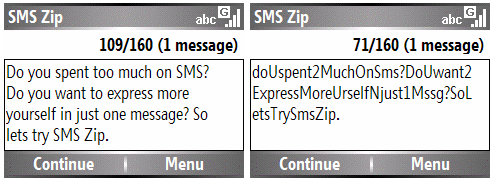
\includegraphics []{Billeder/SMSZIP.png}
\caption {På figuren ses et eksempel på en besked komprimeret af programmet SMS ZIP}
\end{figure}

Denne konkrete besked bliver altså kortet ned fra 109 til 71 tegn. En af fordelene ved dette program er, at modtageren ikke behøver et tilsvarende dekomprimeringsprogram for at kunne læse beskeden. En anden fordel er, at beskeder der ikke overgår en begrænsningen, ikke nødvendigvis bliver komprimeret. Denne løsning har dog en del flere ulemper end fordele. Den åbenlyse ulempe er at beskederne bliver en hel del sværere at læse, og kan være en mulig irritation for mange, når de læser beskeden. En anden klar ulempe er at der bliver brugt en del slang for at gøre ordene kortere, slang såsom tallet '2' i stedet for ordet 'to' eller 'too'. Dette kan bevirke at budskabet er sværere at tage seriøst. Yderligere er det et problem, at programmet kun virker til ældre Windowsphone systemer, og at forkortelserne kun er beregnet til engelsktalende beskeder. Det er derfor, på baggrund af ovenstående, vores vurdering at programmet er en ufuldstændig løsning, og er dermed ikke tilstrækkelig.\cite{download-sms}

En anden eksisterende løsning hedder SMS ZIPPER. Det er på mange punkter et modstridende program i forhold til SMS ZIP. Først og fremmest er det forskelligt da dette er et tabsfrit komprimerings program. Programmet virker på langt de fleste smartphones og er, i modsætning til SMS ZIP, en løsning der komprimerer beskeden hos afsenderen og derefter dekomprimerer beskeden igen hos modtageren. Dette kræver dog at både afsender og modtager har programmet installeret. Programmet starter på modtagerens telefon ligeså snart en komprimeret besked modtages, så beskeden kan læses med det samme uden besvær for læseren. Producenten lover helt op til 480 tegn pr. besked, altså 3 gange så mange tegn som en almindelig SMS. Derudover fungerer programmet til flere sprog, heriblandt dansk, engelsk og tysk.

Dette program bruger en speciel designet algoritme til at komprimere beskederne. De har designet algoritmen direkte med henblik på såkaldte korte beskeder, altså beskeder omkring de 160 tegn. Endvidere bruger programmet også andre kodnings modeller, som kan være beregnet specifikt på bestemte sprog eller typer af beskeder. Dette program har til gengæld også en masse features, som ikke er relevante for komprimering, og heller ikke nødvendigvis relevante for brugeren. Dette inkluderer blandt andet muligheden for at sikre sine beskeder med password, en anden feature er selvdestruerende SMS'er. Hvis brugeren leder efter et program der kun kan komprimere og dekomprimere, så er SMS ZIPPER ikke programmet man leder efter.\cite{smszipper} 

I ovenstående afsnit har vi valgt at kigge nærmere på to vidt forskellige programmer, for at tegne en kontrast mellem en meget simpel og en mere avanceret løsning. Vi ser at de hver især har deres fordele og ulemper, og disse vil vi tage til overvejelse i vores program.